\documentclass[conf]{new-aiaa}
%\documentclass[journal]{new-aiaa} for journal papers
\usepackage[utf8]{inputenc}
\usepackage[super]{nth}

% Load a number of useful packages
\usepackage{longtable,tabularx}
\setlength\LTleft{0pt} 
\usepackage{booktabs}
\usepackage{multirow}
\usepackage{graphicx}
\usepackage{caption}
\usepackage{subcaption}
\usepackage{amsmath,amssymb,amsfonts,amsthm,amsbsy}
\usepackage{bm}
\usepackage{enumerate}
\usepackage{cancel}
%\usepackage[margin=1.0in]{geometry}
\usepackage[colorlinks=true]{hyperref}
\hypersetup{
    colorlinks=true,
    linkcolor=blue,
    filecolor=magenta,      
    urlcolor=blue,
    citecolor=red,
    pdftitle={Sharelatex Example},
    bookmarks=true,
    pdfpagemode=FullScreen,}
%\usepackage{cite}
\usepackage[caption=false,font=footnotesize]{subfig}
\usepackage{float}
\usepackage{color} %red, green, blue, yellow, cyan, magenta, black, white
\definecolor{mydgray}{RGB}{40,44,52}
\definecolor{myred}{RGB}{224,108,117}
\definecolor{mygreen}{RGB}{152,195,121}
\definecolor{myorange}{RGB}{229,192,123}
\definecolor{myblue}{RGB}{97,175,239}
\definecolor{mypurple}{RGB}{198,120,221}
\definecolor{myteal}{RGB}{86,182,194}
\definecolor{mygray}{RGB}{171,178,191}
\usepackage{accents}
\newcommand*{\dt}[1]{\accentset{\mbox{\large\bfseries .}}{#1}}
\newcommand*{\ddt}[1]{\accentset{\mbox{\large\bfseries .\hspace{-0.25ex}.}}{#1}}
\usepackage{tcolorbox}
\tcbuselibrary{skins,xparse,breakable}
\tcbset{breakable}
\usepackage[scientific-notation=true]{siunitx}
\usepackage[capitalize]{cleveref}
\RequirePackage[sort&compress,numbers]{natbib}

%% https://www.sharelatex.com/learn/Code_listing
\usepackage[final]{pdfpages}
\usepackage{subfig}
\usepackage{listings}

\definecolor{codegreen}{rgb}{0,0.6,0}
\definecolor{codegray}{rgb}{0.5,0.5,0.5}
\definecolor{codepurple}{rgb}{0.58,0,0.82}
\definecolor{backcolour}{rgb}{0.97,0.97,0.97}
 
\lstdefinestyle{nonumbers}{
    backgroundcolor=\color{backcolour},   
    commentstyle=\color{codegreen},
    keywordstyle=\color{magenta},
    numberstyle=\tiny\color{codegray},
    stringstyle=\color{codepurple},
    basicstyle=\footnotesize,
    breakatwhitespace=false,         
    breaklines=true,                 
    captionpos=b,                    
    keepspaces=true,                 
    numbers=none,                    
    numbersep=5pt,                  
    showspaces=false,                
    showstringspaces=false,
    showtabs=false,                  
    tabsize=2
}
\lstset{style=nonumbers}

\lstdefinestyle{numbers}{
    backgroundcolor=\color{backcolour},   
    commentstyle=\color{codegreen},
    keywordstyle=\color{magenta},
    numberstyle=\tiny\color{codegray},
    stringstyle=\color{codepurple},
    basicstyle=\footnotesize,
    breakatwhitespace=false,         
    breaklines=true,                 
    captionpos=b,                    
    keepspaces=true,                 
    numbers=left,                    
    numbersep=5pt,                  
    showspaces=false,                
    showstringspaces=false,
    showtabs=false,                  
    tabsize=2
}
\lstset{style=numbers}

% Two more packages that make it easy to show MATLAB code

\usepackage[framed,numbered]{matlab-prettifier}
\lstset{
	style = Matlab-editor,
	basicstyle=\mlttfamily\small,
}

% Say where pictures (if any) will be placed
\graphicspath{{./figures/}}

\title{Modeling of Waves Generated by the 2010 Haiti Earthquake}


\author{Parthiv Kukadia}
\affil{Junior, AE Department, the University of Illinois at Urbana-Champaign}

\begin{document}

\maketitle

\begin{abstract}
This paper describes the modeling process of a 2D harmonic wave using a second order finite difference method. The author was able to use real world data from the 2010 Haiti Earthquake to set boundary conditions for the model and obtain an approximate solution. The approximate solution was compared to the real world data.  
\end{abstract}

\section{Nomenclature and Acronyms}

{\renewcommand\arraystretch{1.0}
\noindent\begin{longtable*}{@{}l @{\quad=\quad} l@{}}
$A,B,C$         & Coefficients\\
$\rho$          & Density \\
$u_{x}, u_{y}$  & \nth{1} order partial derivatives\\
$u_{xx}, u_{yy}$& \nth{2 } order partial derivatives\\
$T$             & Tension\\
$\alpha,\beta$  & Angles\\
$v$             & Wave velocity\\
$t$             & Time\\
BVP             & Boundary Value Problem\\
IVP             & Initial Value Problem\\
NOAA            & National Oceanic and Atmospheric Administration\\
\end{longtable*}}

\section{Introduction}

On January 12, 2010, a magnitude 7.0 earthquake struck Haiti. It was the most devastating natural disaster in Haiti's history:
\begin{itemize}
    \item an estimated 250,000 people died
    \item at least 300,000 people injured
    \item 5 million people displaced
    \item nearly 4,000 schools damaged or destroyed
    \item at the time of the earthquake, 70\% of the population lived below the poverty line \cite{haiti}
\end{itemize}
\bigskip
\par
When the earthquake struck, computer models predicted that a tsunami would hit the nation's south shore — but with a height of just 20 centimetres \cite{tsunami}. However, it was later discovered at least two \SI{3}{meter} tsunamis struck Haiti's shores knocking down building walls and washing boats ashore. What if better models existed and could have helped saved lives or given an earlier warning? That is the motivation behind our paper and model.

\section{The Acoustic Wave Equation}
\subsection{The Basic 1D Wave Equation}
The partial differential equation
\begin{align}
    Au_{xx}+2Bu_{xy}+Cu_{yy} =0
\end{align}
can be classified as elliptic, parabolic, or hyperbolic according to the matrix
\begin{align*}
    \begin{bmatrix}
    A & B\\
    B & C
    \end{bmatrix}
\end{align*}
\begin{itemize}
    \item $AC > B^2\Longrightarrow$
    elliptic BVP: steady state equations (Laplace's equation)
    \item $AC = B^2\Longrightarrow$
    parabolic IVP: heat/diffusion equations
    \item $AC < B^2\Longrightarrow$
    hyperbolic IVP: wave/convection equations
\end{itemize}
In one spatial dimension (1D), the simplest form the wave equation takes is
\begin{align}
    \frac{\partial^2 u}{\partial t^2} &= c^2 \frac{\partial^2 u}{\partial x^2} \label{eq:simpleform}
\end{align}
where $c$ is a constant referred to as the wave speed.\\ \\
A general solution to the wave equation in which the displacement varies only in the direction of propagation, e.g. a plane wave travelling along the x-axis:
\begin{align}
    u(x,t)= g(x - ct) + h (x + ct) \label{eq:simplesol}
\end{align}
where $g$ and $h$ and any single value function. This shows half the wave travels in one direction and half of the wave travels in the other direction.\\ \\
Simple substitution shows \cref{eq:simplesol} is a solution to \cref{eq:simpleform}
\begin{equation*}
    \begin{split}
        \frac{\partial u}{\partial t} &= -cg^\prime(x-ct) + ch^\prime(x+ct)\\
        \frac{\partial^2 u}{\partial t^2} &= -c^2g^{\prime\prime}(x-ct) + c^2h^{\prime\prime}(x+ct)\\
    \end{split}
    \hspace{2cm}
    \begin{split}
        \frac{\partial u}{\partial x} &= g^\prime (x-ct) + h^\prime(x+ct)\\
        \frac{\partial^2 u}{\partial x^2} &= g^{\prime\prime} (x-ct) + h^{\prime\prime}(x+ct)\\
    \end{split}
\end{equation*}
\begin{align*}
    \bm{\therefore} \hspace{.25cm} \frac{\partial^2 u}{\partial t^2} &= c^2 \frac{\partial^2 u}{\partial x^2}
\end{align*}
\subsection{Basic 2D Wave Equation}
Stepping up a notch, we can model the the motion of an ideal membrane in three dimensions using the 2D wave equation.\\
Assume we have a membrane at rest in the xy plane of an xzy coordinate system. We make a number of assumptions about it:
\begin{itemize}
    \item has a constant density $\rho$
    \item is flexible
    \item is fixed along its boundary
    \item any tension, $T$, applied to it is uniform and constant
    \item out of plane deflections are small
\end{itemize}
\begin{figure}[H]
    \begin{center}
    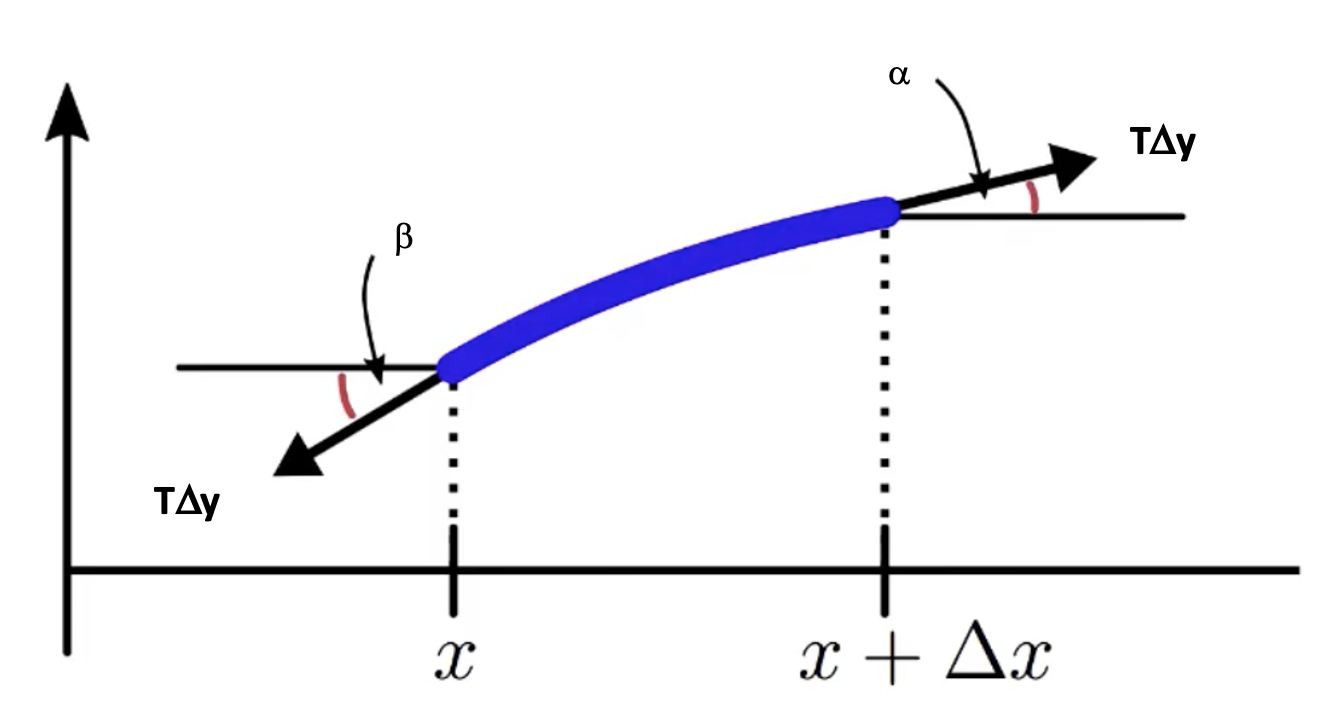
\includegraphics[width =.4\linewidth]{figures/zx_plane.png}
    \caption{Sideview of Membrane}
    \label{fig_zx}
    \end{center}
\end{figure}
We let 
\begin{align}
    u(x,y,t) &= \text{the vertical deflection of the membrane from $(x,y)$ at time $t$}
\end{align}
We apply a tension, $T$, to a small section of the membrane so there is a deflection. Looking at this small section from the xz plane as shown in \cref{fig_zx}, we can sum the forces acting in the horizontal direction on the left and right sides of the membrane.
\begin{align}
    \sum \text{Forces}_{horiz}^{left/right} &= T\Delta y \cos(\beta) - T\Delta y \cos(\alpha)
\end{align}
\\
using small angle assumption drives $cos \longrightarrow 1$
\begin{align}
    \therefore \sum \text{Forces}_{horiz}^{left/right} &= 0
\end{align}
\\
Similarly, for the forces acting in the vertical direction
\begin{align}
    \sum \text{Forces}_{vert}^{left/right} &= T\Delta y \sin(\beta) - T\Delta y \sin(\alpha)
\end{align}
\\
using small angle assumption $sin \theta \approx \theta \approx tan \theta$
\begin{align}
    \sum \text{Forces}_{horiz}^{left/right} &= 0\\[8pt]
    \sum \text{Forces}_{vert}^{left/right} &= T\Delta y [\tan(\beta) - \tan(\alpha)]
\end{align}
\\
Rewriting $tan(\beta)$ and $tan(\alpha)$,
\begin{align}
    \tan(\beta) &= \frac{\partial u}{\partial x }\Bigr|_{\substack{x=x+\Delta x\\y=y_1 \in [y,y+\Delta y]}} = u_{x}(x+\Delta x, y_1)\\[10pt]
    tan(\alpha) &= \frac{\partial u}{\partial x }\Bigr|_{\substack{x=x\\y=y_2 \in [y,y+\Delta y]}} = u_{x}(x, y_2)
\end{align}
\\
We arrive at 
\begin{align}
    \sum \text{Forces}_{vert}^{left/right} &= T\Delta y[u_x (x+\Delta x,y_1) - u_x (x,y_2)]
\end{align}
\\
A similar process is used on the membrane along the yz plane in order to derive
\begin{align}
    \sum \text{Forces}_{vert}^{front/back} &= T\Delta x[u_y (x_1,y+\Delta y) - u_y(x_2,y)]
\end{align}
\\
Using Newton's Second Law,
\begin{align}
    ma &= \sum \text{Forces}_{vert}\\[8pt]
    \rho \Delta x \Delta y \frac{\partial^2 u}{\partial t^2} & = T\Delta y[u_x (x+\Delta x,y_1) - u_x (x,y_2)] + T\Delta x[u_y (x_1,y+\Delta y) - u_y(x_2,y)]\\[8pt]
    \frac{\partial^2 u}{\partial t^2} &= \frac{T}{\rho} \Bigg[\frac{u_x (x+\Delta x,y_1) - u_x (x,y_2)}{\Delta x} + \frac{u_y (x_1,y+\Delta y) - u_y(x_2,y)}{\Delta y}\Bigg]\\[8pt]
    \frac{\partial^2 u}{\partial t^2} &= \frac{T}{\rho} \Bigg(\frac{\partial^2 u}{\partial x^2}+ \frac{\partial^2 u}{\partial y^2}\Bigg)\\[8pt]
    \therefore \frac{\partial^2 u}{\partial t^2} &= c^2 \Bigg(\frac{\partial^2 u}{\partial x^2}+ \frac{\partial^2 u}{\partial y^2}\Bigg) \label{eq:final2}
\end{align}

\subsection{Problem Application}
The measuring stations of the 2010 Haiti earthquake provided by the National Oceanic and Atmospheric Administration (NOAA) were all placed in sea near the coast of Haiti. Because our data was collected in the water near the earthquake site, we modeled a harmonic wave. A harmonic wave is the type of wave that takes place before the earthquake hits land. The wave is also called a P-wave because it is the primary wave before there is large damage on land.

\section{Numerical Methods}
\subsection{Description and Derivation of Method}
We used a \nth{2} order central finite difference scheme in order to approximate the harmonic wave. We took \cref{eq:final2} and put it into this form
\begin{align}
    u(x,y,t) &= v^2 \Bigg(\frac{\partial^2 u}{\partial x^2}+ \frac{\partial^2 u}{\partial y^2}\Bigg)
\end{align}
applied a set of general solutions,
\begin{align}
    u(x,t) &= a \cos(\omega t - kx)\\
    u(y,t) &= a \sin(\omega t - ky)
\end{align}
we arrived at the approximate solution equation
\begin{align}
    u(x,y,t) &= -v^2(a \sin(\omega t - ky) + a \cos(\omega t - kx))
\end{align}
\subsection{Justification}
In order for us to know if our numerical method is reliable, it is vitally important for us to have a valid way to verify our results. There can actually be no better comparison for our model than using data collected by NOAA. We ran error differences between out model and the NOAA data, which are shown later in the report.

\subsection{Initial and Boundary Conditions}
We used the NOAA data to set the initial conditions and boundary conditions for our exact solution model and approximate solution model. That is, both models received the same set of initial conditions and boundary conditions. Certain parameters were also set for the exact model: frequency, wave velocity, omega and phi. Parameters for the approximate solution were based on using the \nth{2} order central finite difference method. We discovered we had to implement a Courant-Friedrich Levy (CFL) condition Value in order to make our approximate solution work. Basically, the Courant-Friedrich Levy is a condition in numerical equation solving which states that, given a space discretization, a time step bigger than some computable quantity should not be taken. The condition can be viewed as a sort of discrete "light cone" condition, namely that the time step must be kept small enough so that information has enough time to propagate through the space discretization \cite{CFL}. We had to adjust our approximate solution model to reflect the CFL condition.

% \subsection{Demonstration of Correct Implementation}

%\section{Application Of The Wave Equation}

\subsection{Data Acquisition}
One of the challenges to the task of approximating a wave and comparing it to a real seismic wave was finding accurate data for a real wave in the form of numbers instead of a graph. For the Haiti 2010 earthquake, NOAA had measuring stations close to the Haiti coast in the Caribbean Sea and the Atlantic Ocean. These measuring stations, referred to as Deep-ocean Assessment and Reporting of Tsunami (DART) buoys, are able to measure and record changes in ground displacements. A recording sample of DART 41420 is shown in \cref{fig_dart41420}.
\begin{figure}[H]
    \begin{center}
    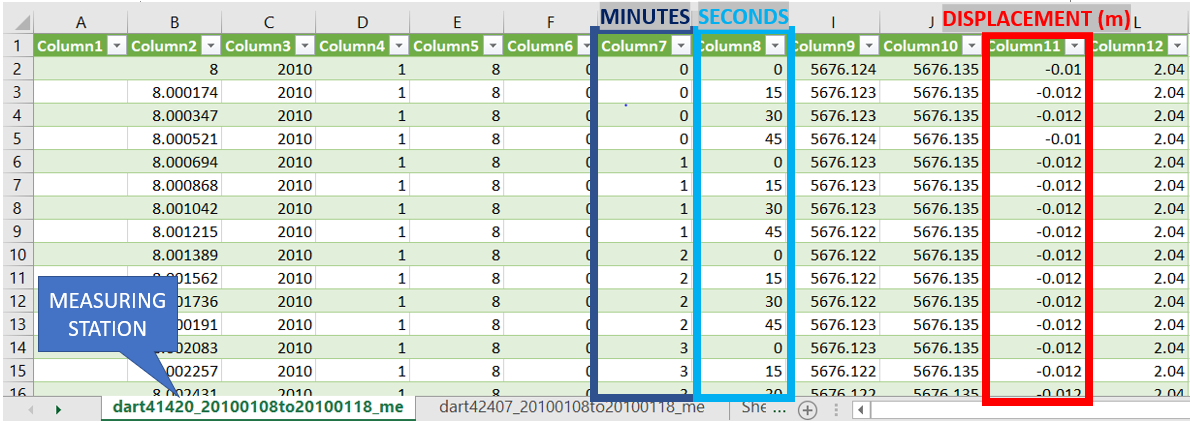
\includegraphics[width =1\linewidth]{figures/XCEL DATA.PNG}
    \caption{Raw data from DART 41420 during Haiti 2010 Earthquake}
    \label{fig_dart41420}
    \end{center}
\end{figure}

NOAA does not have measuring stations on the land of Haiti so we used the closed measuring stations which were the DART 42407 (358 miles from Port au Prince) and the DART 4120 (452 miles from Port au Prince). Although these stations are seemingly far, the earthquake would be felt at the stations. For reference, a magnitude 5.5 earthquake can be felt over 300 miles from the epicenter and the Haiti earthquake was a magnitude 7.0 on the Richter Scale.\cref{fig_dartlocation} shows DART locations.

\begin{figure}[H]
    \begin{center}
    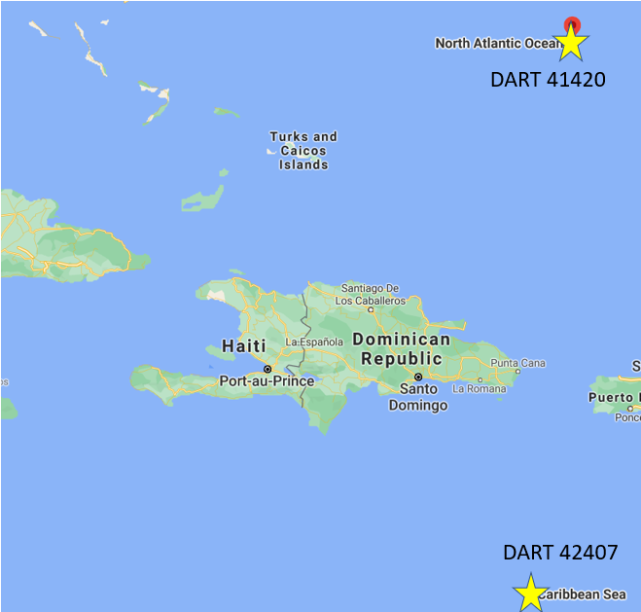
\includegraphics[width =.7\linewidth]{figures/ground stations.png}
    \caption{DART 42407 and DART 41420 Locations with respect to Haiti}
    \label{fig_dartlocation}
    \end{center}
\end{figure}

\subsection{Modeling}
To provide a model of the seismic wave equation, the numerical methods were implemented into MATLAB. Instead of a typical 1D plot, the MATLAB outputs three 2D graphs that change in time. One is for the approximation, another for the real data, and the final for the error. The conditions in MATLAB depend on amplitude, velocity, frequency and phase angle of the wave. The amplitude of the approximation was created going off of the amplitude at t=0, and the displacement for times after that were created using the Finite Difference Method. The amplitude of the exact method was created and updated using the NOAA data given. 

The inputs in the MATLAB code are the wave displacement and velocity. The displacements are labeled as $u\_app$ and $u\_ex$ for the approximation displacement and exact displacement from the observed data, respectively. 

The velocity of the Haiti earthquake was calculated by finding the impact area of the earthquake, the distance traveled by an earthquake wave, and the duration the wave lasted. All of these values are easily accessible as they are measured with every earthquake. With an impact radius of 6180.38 meters and an impact duration of 35-60 seconds, (which we approximated to be 40 seconds) the estimated wave velocity was approximated to be \textbf{154.51 meters per second}. 

The output displays an approximation for the wave over a .4 x 1 meter area of space. The model will generate a screenshot of the plot at every time there is no error, or the wave generated by using measured values as the input was equal to the wave generated by using the second order finite difference method. The screenshots should theoretically be when the model is most accurate. The simulation shows the wave for every .01 hours from t = 0 hours to t = .9 hours. 

A 1D model was also created for a fixed y value. The 1D model shows the change in wave displacement as the x value changes. A screenshot was produced every time the 

\begin{figure}[H]
    \begin{center}
    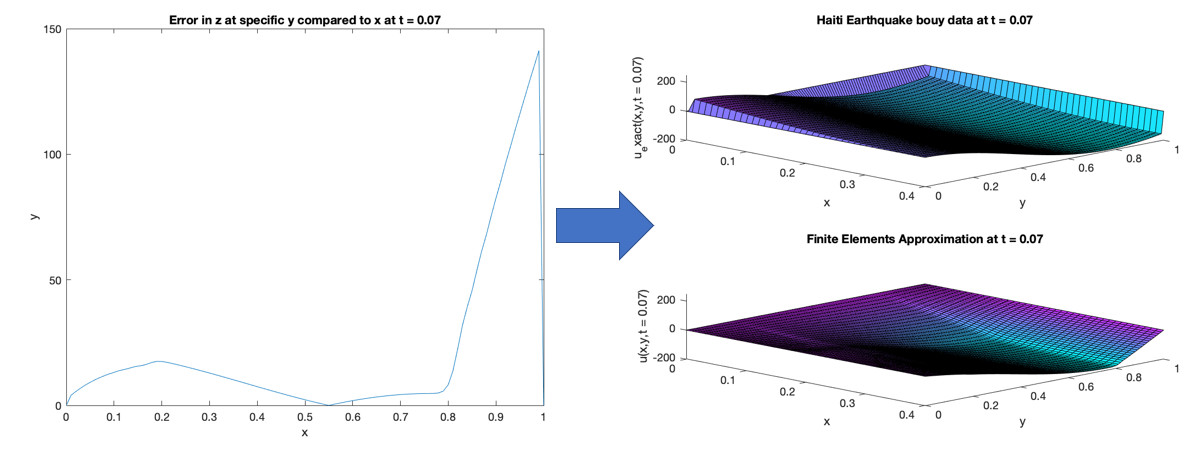
\includegraphics [width= 1\linewidth]{figures/1d2d.png}
    \caption{MATLAB Output 1D Model (left) And 2D Model (right)}
    \label{fig_1d2d}
    \end{center}
\end{figure}



\subsection{Approximation Significance}
It may initially seem illogical to approximate a 2-dimensional wave when we already are given the data. However, approximating the wave using a harmonic wave in a 2-dimensional space and comparing that data to real data can have a significant impact.

First, knowing the shape of the wave and how the wave propagates in space can allow us to predict which areas will be the most hazardous during an earthquake. With this information, we can more properly warn people and distribute resources during a crisis. Having observed data in addition to a hypothesis is the best way to see how closely the wave follows the expected trajectory.

Next, studying seismic waves and their movement is essential for geologists to study the Earth's core and its materials. With more knowledge about the Earth's core, geologists could potentially predict earthquakes and even when one will happen. 


\section{Results}
\subsection{Convergence and Method Justification}
The 2D Finite Difference Method was chosen during this analysis because it has an error on the order of $\Delta t^2$. Every problem that tried to solve the seismic wave equation used the finite difference method. The method was straightforward and easily adaptable to the 2d scenario. 

A complete convergence analysis for a 2-dimensional problem is not feasible. However, we are able to tell by the error plots for which values the wave has the least amount of error. 

\subsection{Wave Approximation vs. Real Data}

\begin{figure}[H]
    \begin{center}
    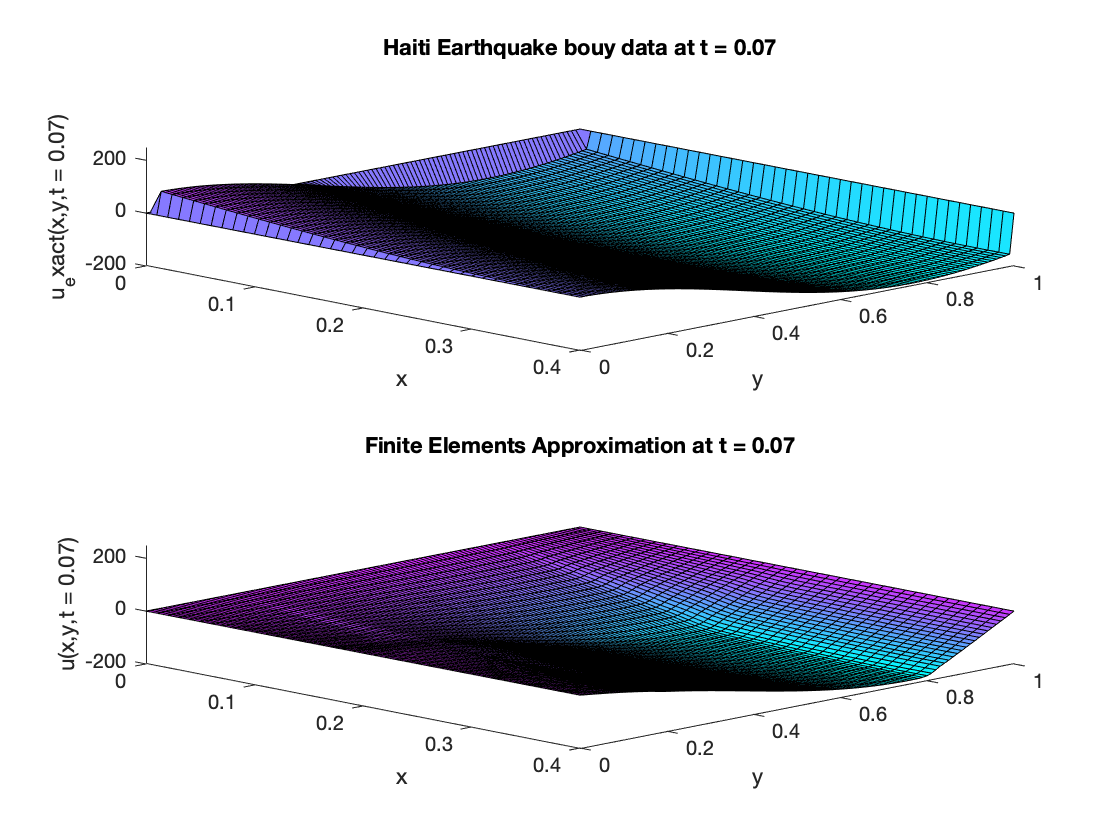
\includegraphics [width= 1\linewidth]{figures/ExactandApprox_t007.png}
    \caption{Exact and Approximate Solutions at $t=0.07s$}
    \label{fig_t007}
    \end{center}
\end{figure}

\begin{figure}[H]
    \begin{center}
    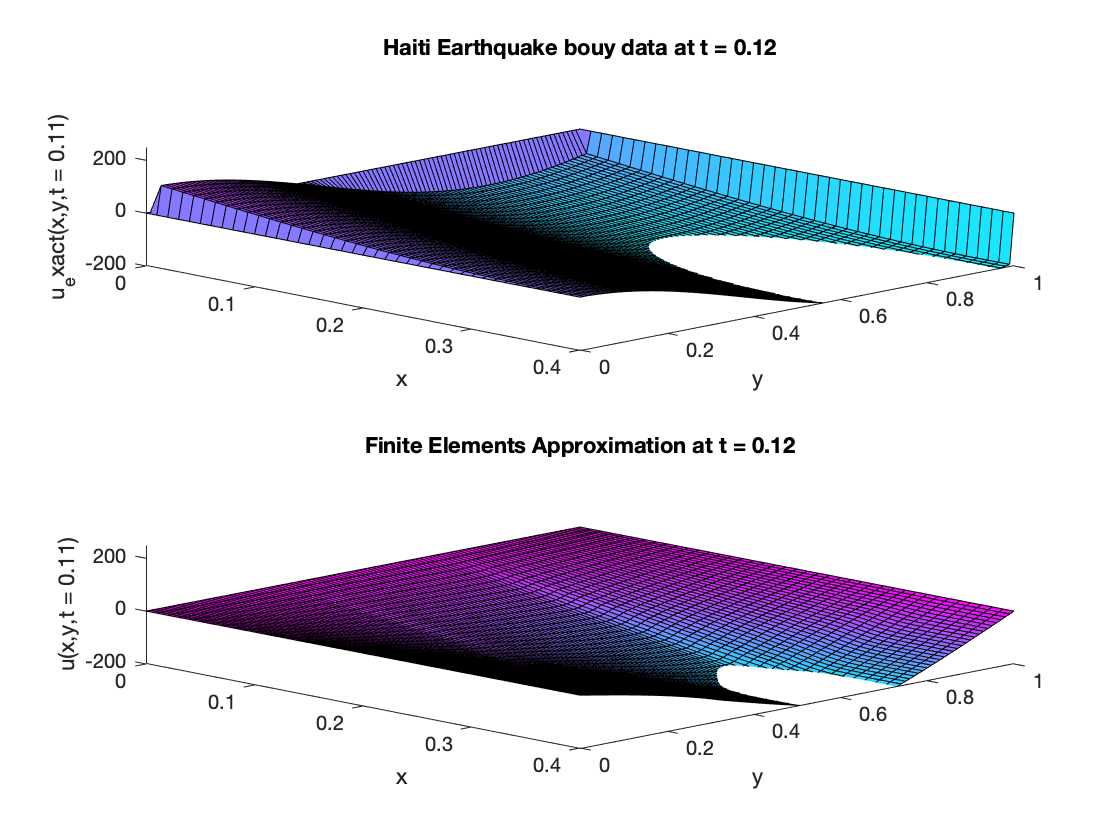
\includegraphics [width= 1\linewidth]{figures/ExactandApprox_t012.png}
    \caption{Exact and Approximate Solutions at $t=0.12s$}
    \label{fig_t012}
    \end{center}
\end{figure}

\begin{figure}[H]
    \begin{center}
    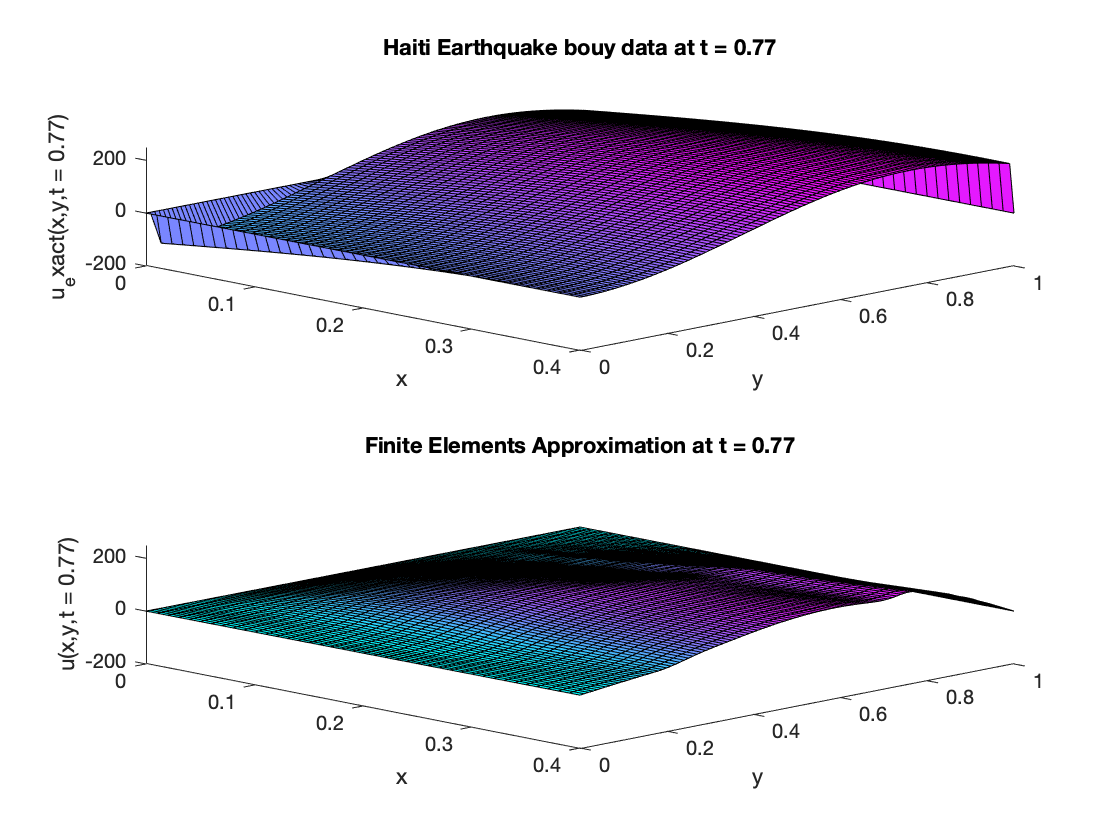
\includegraphics [width= 1\linewidth]{figures/ExactandApprox_t077.png}
    \caption{Exact and Approximate Solutions at $t=0.77s$}
    \label{fig_t077}
    \end{center}
\end{figure}

\begin{figure}[H]
    \begin{center}
    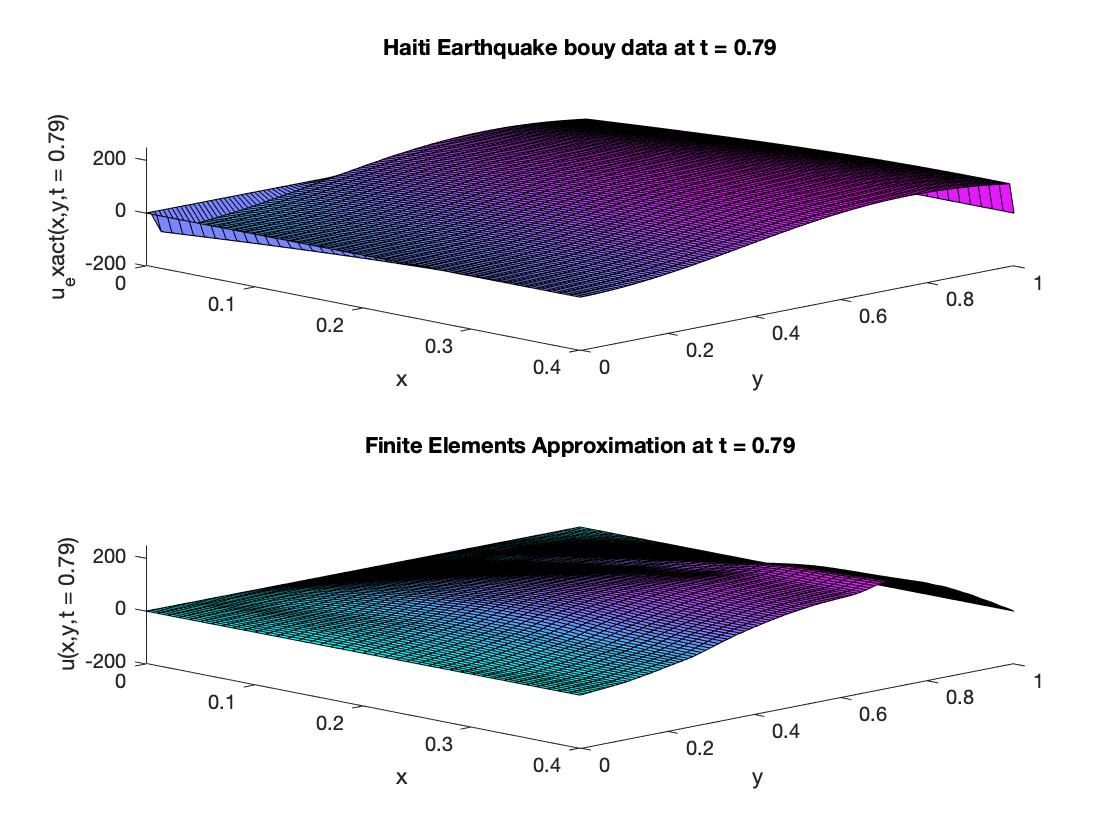
\includegraphics [width= 1\linewidth]{figures/ExactandApprox_t079.png}
    \caption{Exact and Approximate Solutions at $t=0.79s$}
    \label{fig_t079}
    \end{center}
\end{figure}

\begin{figure}[H]
    \begin{center}
    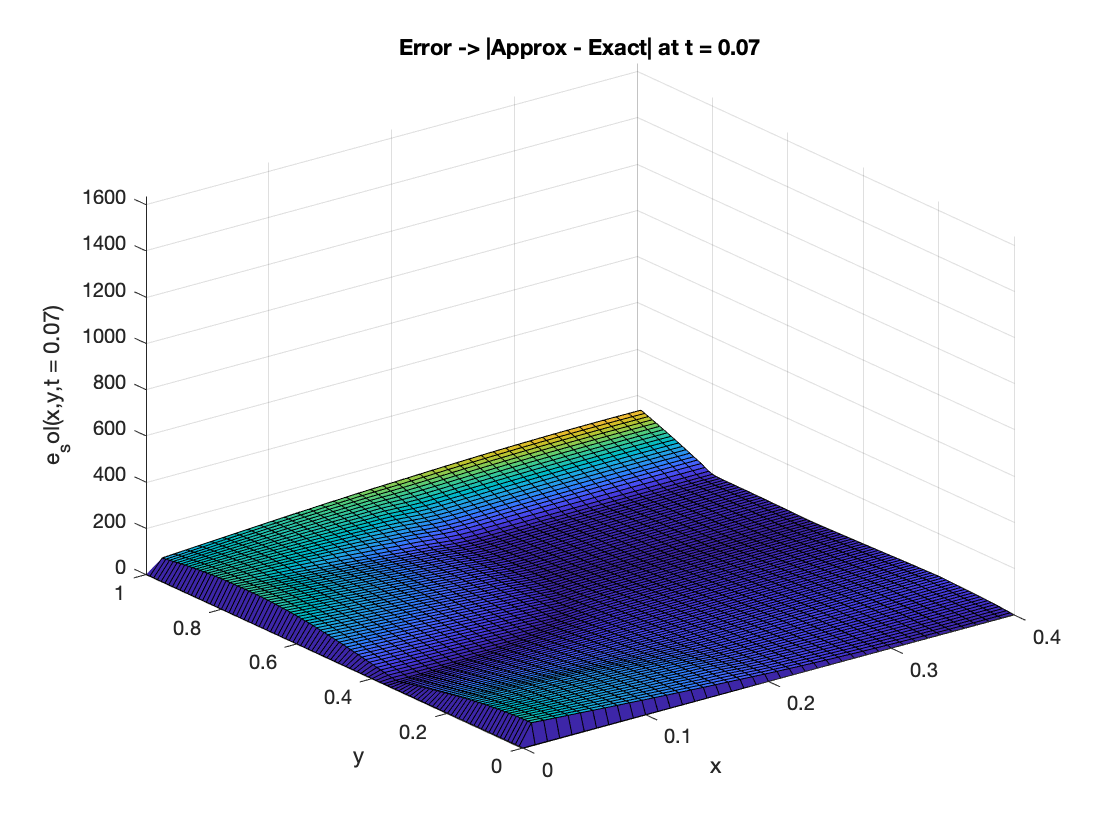
\includegraphics [width= .8\linewidth]{figures/Error_t007.png}
    \caption{Error at $t=0.07s$}
    \label{fig_errt007}
    \end{center}
\end{figure}

\begin{figure}[H]
    \begin{center}
    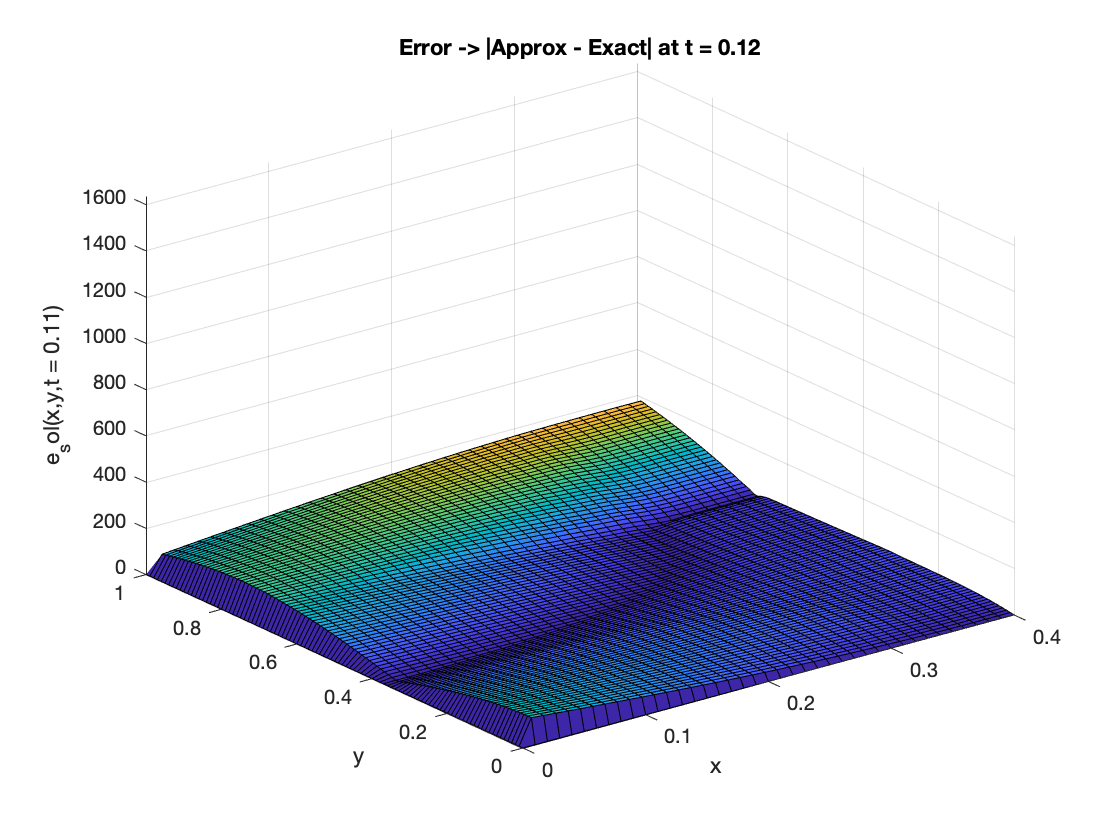
\includegraphics [width= .8\linewidth]{figures/Error_t012.png}
    \caption{Error at $t=0.12s$}
    \label{fig_errt012}
    \end{center}
\end{figure}

\begin{figure}[H]
    \begin{center}
    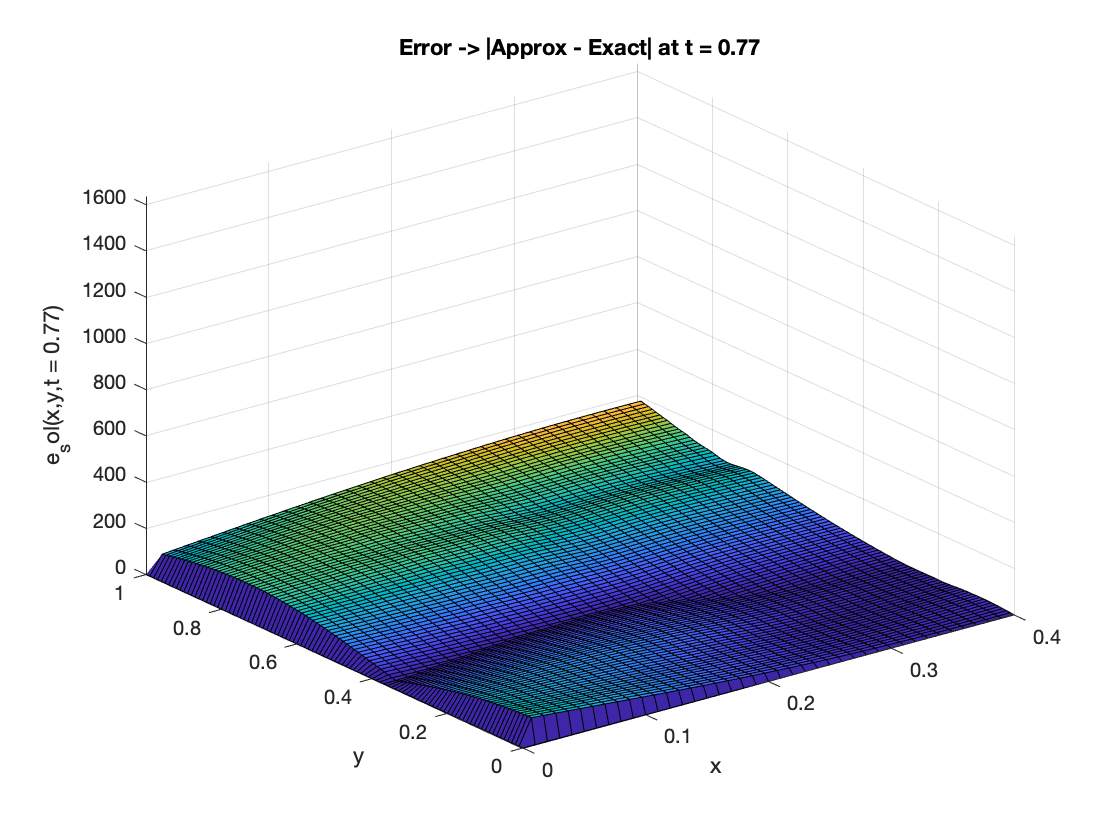
\includegraphics [width= .8\linewidth]{figures/Error_t077.png}
    \caption{Error at $t=0.77s$}
    \label{fig_errt077}
    \end{center}
\end{figure}

\begin{figure}[H]
    \begin{center}
    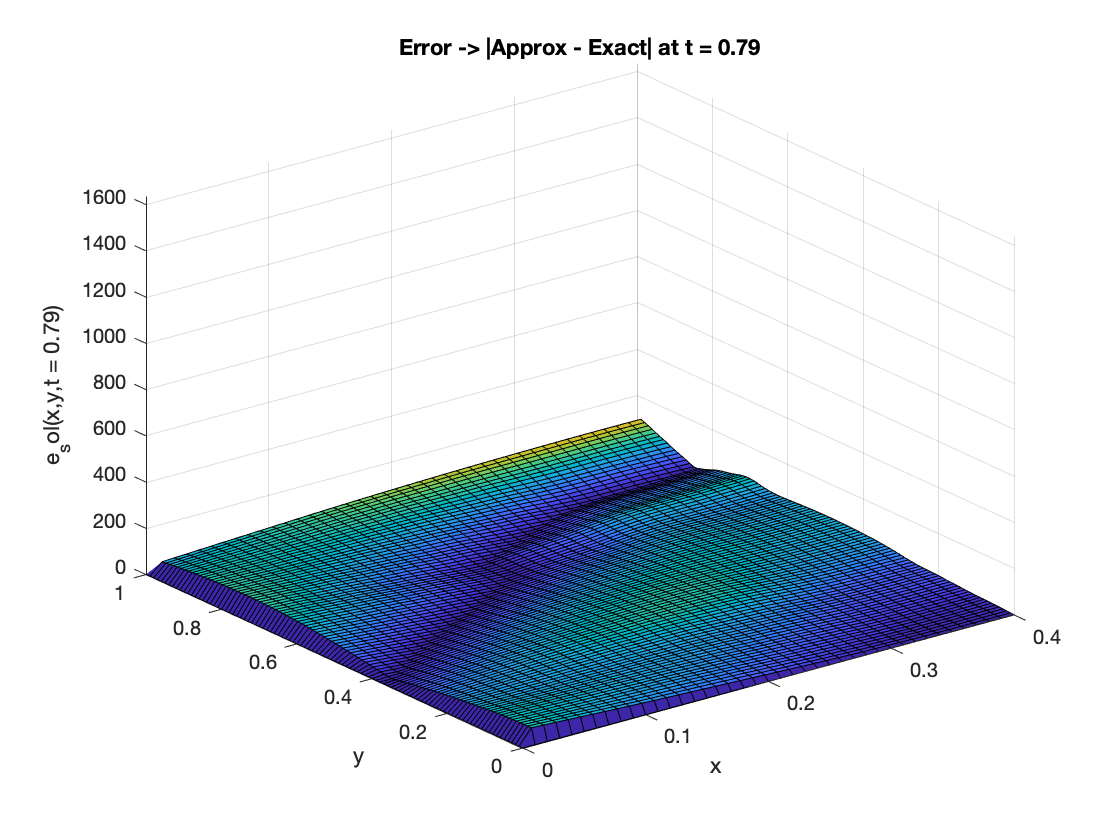
\includegraphics [width= .8\linewidth]{figures/Error_t079.png}
    \caption{Error at $t=0.79s$}
    \label{fig_errt079}
    \end{center}
\end{figure}


\subsection{1D Error Plots}

\begin{figure}[H]
    \begin{center}
    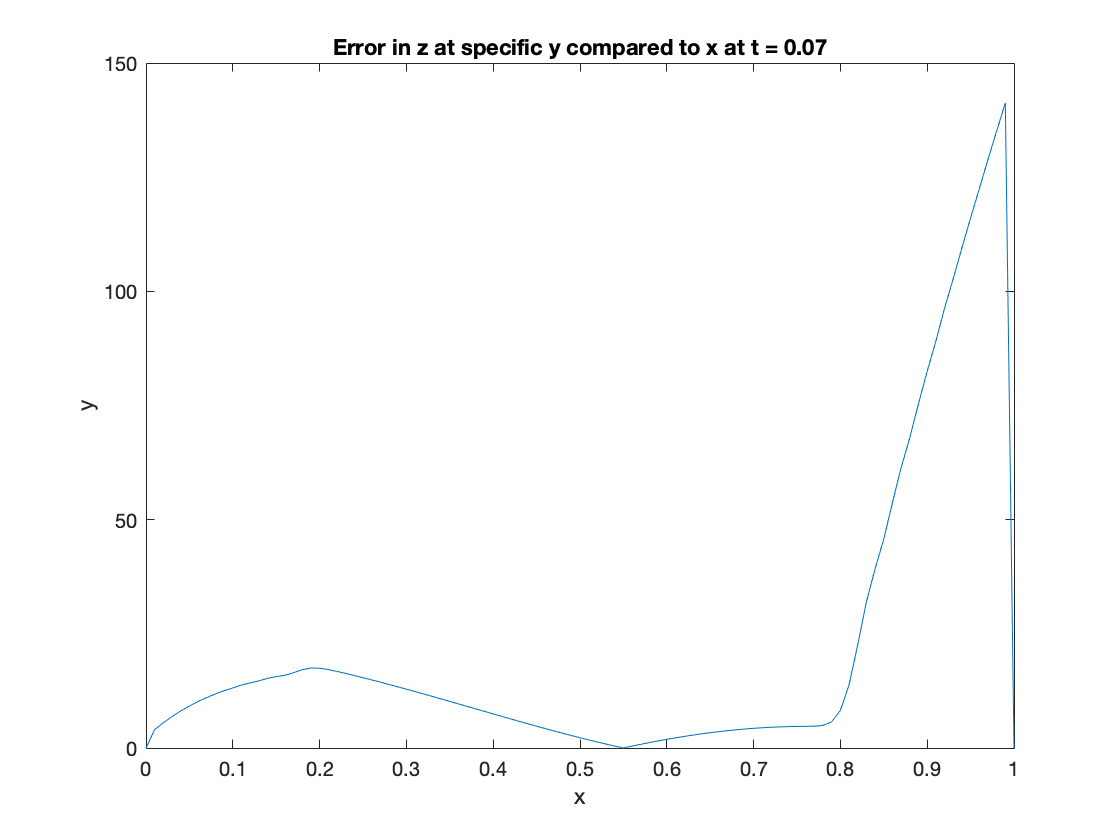
\includegraphics [width= .7\linewidth]{figures/error_at_specific_y_t007.png}
    \caption{1D Error at $t=0.07s$}
    \label{fig_1d07}
    \end{center}
\end{figure}

\begin{figure}[H]
    \begin{center}
    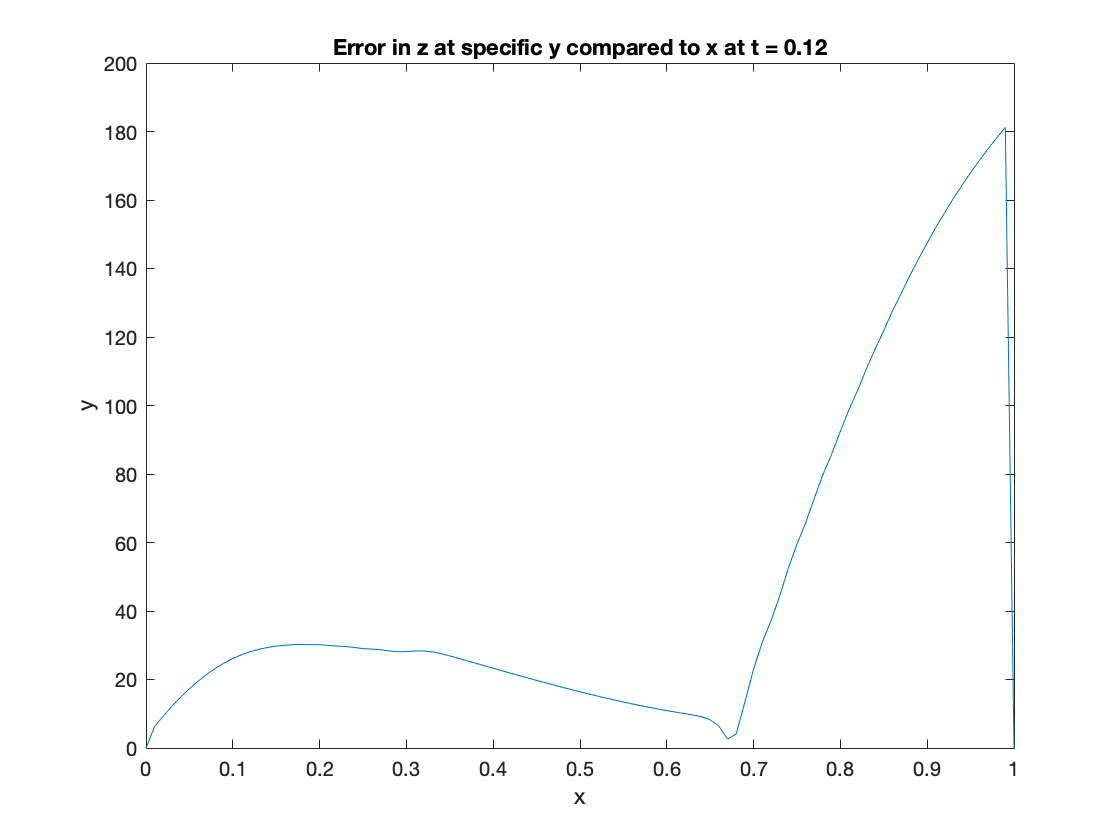
\includegraphics [width= .7\linewidth]{figures/error_at_specific_y_t012.png}
    \caption{1D Error at $t=0.12s$}
    \label{fig_1d12}
    \end{center}
\end{figure}

\begin{figure}[H]
    \begin{center}
    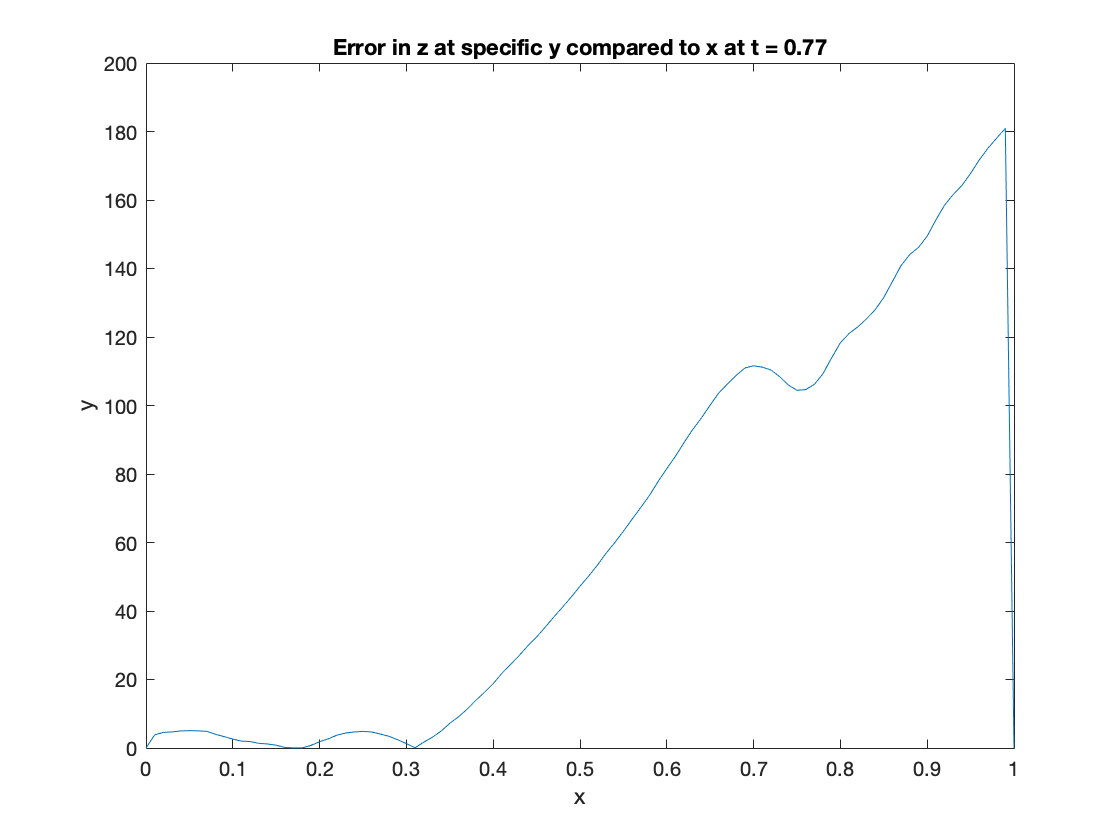
\includegraphics [width= .7\linewidth]{figures/error_at_specific_y_t077.png}
    \caption{1D Error at $t=0.77s$}
    \label{fig_1d77}
    \end{center}
\end{figure}

\begin{figure}[H]
    \begin{center}
    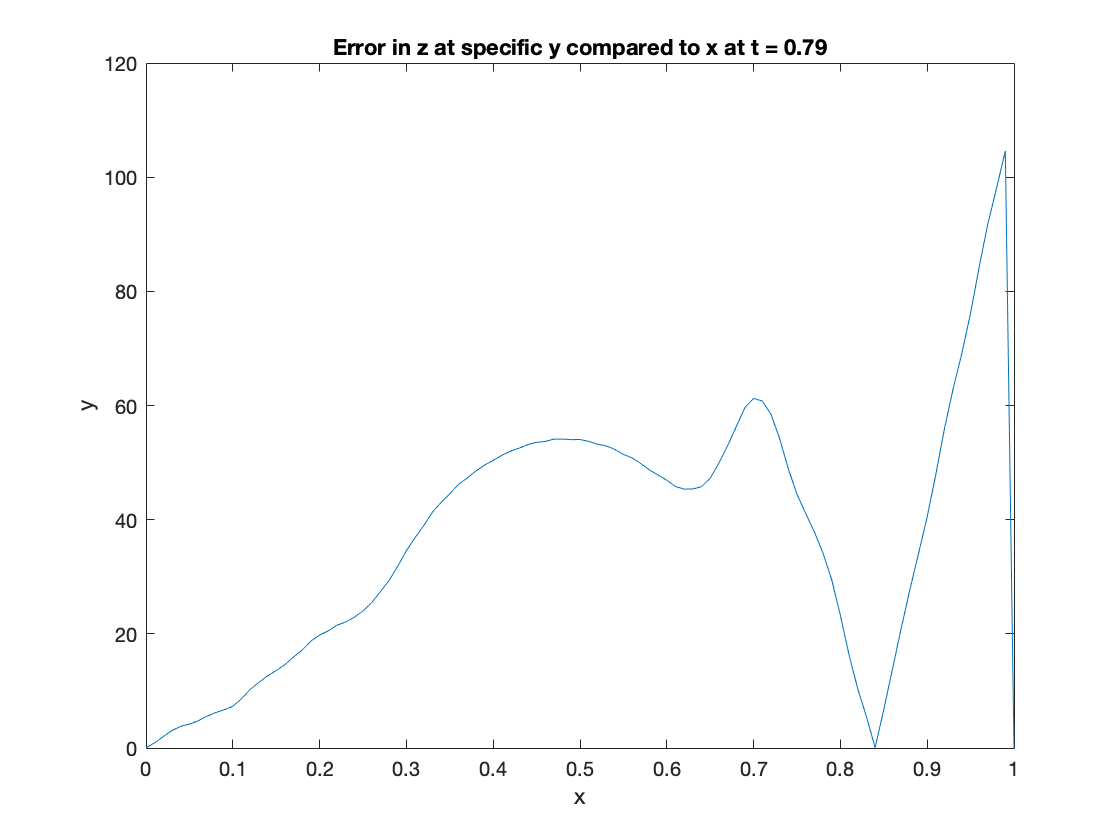
\includegraphics [width= .7 \linewidth]{figures/error_at_specific_y_t079.png}
    \caption{1D Error at $t=0.79s$}
    \label{fig_1d79}
    \end{center}
\end{figure}

\subsection{Results analysis}
The waves as pictured above show a .4 x 1 meter rectangle with its displacement. The displacement is rather large as 

\subsection{Error analysis}
The waves produced give a useful visual for what the ground would look like during an earthquake. This is very useful for analyzing how earthquakes move and the effect tectonic plates have on an earthquake. Even though the result gives a clean looking visual, the errors are rather high when approximating the earthquake displacement compared to the measured data.

Reasons for this could be that the earthquake did not follow a perfect wave. This reason for the error is very likely because the data was given over a short period of time that may not be long enough to fully model a wave. 


Another reason for high errors could be from inconsistencies in our boundary conditions or initial conditions. When approximating, we made many assumptions like the wave velocity for the entire wave and the amplitude at an arbitrary time for the initial amplitude when using the finite difference method.

A third reason for the high errors could be from the measuring station location. The measuring station was not near the epicenter of the earthquake and thus the wave would likely be weaker and may not follow the wave equation as closely. 

Finally, the large errors can come from the model being 2-dimensional instead of 1-dimensional. In the error plots, the error is much smaller in some areas rather than others. Even with a large error at some points, the approximation graph has the same overall shape as the exact graph. This means even with errors that can peak at 200 meters, the overall shape can be determined from the approximation and the purpose of the approximation is not void. 

\section{Conclusion}
Having access to actual data from the Haiti 2010 earthquake really allowed us to generate a pretty well behaved approximate solution. The \lstinline{meshgrid} and \lstinline{surf} commands in \lstinline{MATLAB} were the linchpin between our solution and some awesome 3D animated plots. Although there was noticeable error as shown in our error plots, we still modeled a 2D wave equation that reflected real world data. The finite difference method proved to be a useful method for approximating the wave equation in 2d space and determining the displacement. The finite difference method was able to accurately predict the overall shape of the wave when compared to observed measured data. This data and method for approximating earthquakes can be useful for determining how earthquakes move and where the displacement will be. This is useful for determining materials at the Earth's core and for warning citizens in areas with a large risk of earthquakes. 

\newpage
\section*{Appendix}
\subsection{Code}
\lstinputlisting[style=Matlab-editor]{code/HarmonicWave2D_Haiti_2010.m}

\newpage
\bibliography{sources}

\end{document}
